\documentclass{article}
\usepackage[T1]{fontenc}
\usepackage{lmodern}
\usepackage{graphicx}
\usepackage{amsmath,amssymb}
\usepackage[a4paper,margin=2cm]{geometry}
\usepackage[absolute,overlay]{textpos}
\setlength{\TPHorizModule}{1mm}
\setlength{\TPVertModule}{1mm}
\usepackage[indonesian]{babel}
\usepackage{hyperref}
\setlength{\emergencystretch}{2em}
\title{03-Kriptografi-klasik-bagian1-(2026)}
\author{pdf\_ppt\_to\_latex}
\date{}

\begin{document}

% --- unit llm 1 ---
% === Halaman 1 (llm) ===

\begin{center}
Bahan kuliah IF4020 Kriptografi

\Huge \textcolor{red}{03 -- Kriptografi Klasik}
\Large \textcolor{red}{(Bagian 1)}

\vspace{10mm}

\large Oleh: Rinaldi M

\vspace{20mm}

\textbf{Program Studi Teknik Informatika}\\
\textbf{Sekolah Teknik Elektro dan Informatika}\\
\textbf{Institut Teknologi Bandung}\\
\textbf{2026}
\end{center}

% deskripsi: Ilustrasi kunci kriptografi klasik berupa silinder logam dengan cincin huruf yang dapat diputar (cipher disk/cylinder).
% bbox normalisasi: [0.0470, 0.4520, 0.2860, 0.7090]
\begin{textblock*}{50.19mm}(9.87mm,134.24mm)
\noindent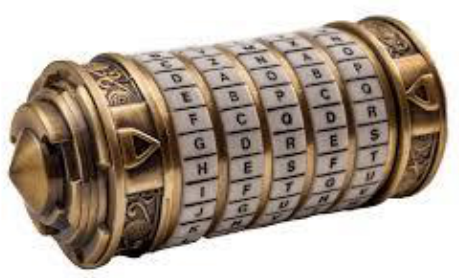
\includegraphics[width=50.19mm,height=76.33mm]{images/llm/page_001_img_01.png}%
\end{textblock*}

\newpage

% --- unit llm 2 ---
% === Halaman 2 (llm) ===

\section*{Pendahuluan}

\begin{itemize}
    \item Kriptografi klasik (\textit{classical cryptography}) merupakan kriptografi yang sudah tua, sudah ada sejak ribuan tahun yang lalu hingga ditemukan komputer digital
    \item \textit{Cipher} pada kriptografi klasik, dinamakan \textit{cipher} klasik, (\textit{classical cipher}) hanya memproses pesan dari huruf-huruf alfabet saja
    \item Menggunakan alat tulis pena dan kertas saja, belum ada komputer
    \item Termasuk ke dalam jenis kriptografi kunci-simetri
\end{itemize}

\begin{itemize}
    \item Tiga alasan mempelajari kriptografi klasik:
    \begin{enumerate}
        \item Memahami konsep dasar kriptografi.
        \item Sebagai dasar algoritma kriptografi modern.
        \item Untuk memahami kelemahan sistem \textit{cipher}.
    \end{enumerate}
\end{itemize}

\newpage

% --- unit llm 3 ---
% === Halaman 3 (llm) ===

\begin{itemize}
  \item \textit{Cipher} di dalam kriptografi klasik disusun oleh dua teknik dasar:
  \begin{enumerate}
    \item \textbf{Teknik substitusi}: mengganti huruf plainteks dengan huruf cipherteks.
  \end{enumerate}
\end{itemize}

\vspace{10mm}

\begin{itemize}
  \item[] Contoh: \quad Plainteks: \texttt{MENGANTUK} \\ Cipherteks: \texttt{CQBSIBONW}
\end{itemize}

\vspace{10mm}

\begin{enumerate}
  \setcounter{enumi}{1}
  \item \textbf{Teknik transposisi}: mengubah susunan atau posisi huruf plainteks menjadi susunan huruf cipherteks. \\ Disebut juga teknik \textit{scrambling}, permutasi, atau pengacakan \\ Contoh: \quad Plainteks: \texttt{MENGANTUK} \\ Cipherteks: \texttt{TNEAKMNGU}
\end{enumerate}

% deskripsi: Tabel pemetaan substitusi huruf alfabet dari Plainteks ke Cipherteks
% bbox normalisasi: [0.1350, 0.2370, 0.9500, 0.3480]
\begin{textblock*}{171.15mm}(28.35mm,70.39mm)
\noindent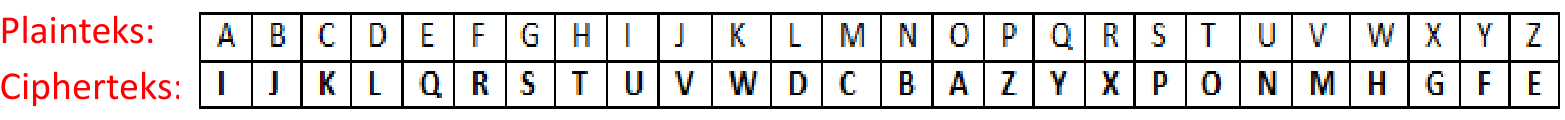
\includegraphics[width=171.15mm,height=32.97mm]{images/llm/page_003_img_01.png}%
\end{textblock*}

\newpage

% --- unit llm 4 ---
% === Halaman 4 (llm) ===

\begin{itemize}
  \item Oleh karena itu, dikenal dua macam \textit{cipher} di dalam kriptografi klasik:
  \begin{enumerate}
    \item \textit{Cipher} Substitusi (\textit{substitution Cipher})
    \begin{itemize}
      \item metode enkripsi dan dekripsi menggunakan teknik substitusi
    \end{itemize}
    \item \textit{Cipher} Transposisi (\textit{transposition Cipher})
    \begin{itemize}
      \item metode enkripsi dan dekripsi menggunakan teknik transposisi
    \end{itemize}
  \end{enumerate}
  \item Kombinasi kedua teknik tersebut membentuk \textit{product cipher} atau \textit{super enkripsi}
  \[ 
    product\ cipher = cipher\ substitusi + cipher\ transposisi
  \]
\end{itemize}

\newpage

% --- unit llm 5 ---
% === Halaman 5 (llm) ===

% (tidak ada teks dari model)

% deskripsi: Diagram hierarki Kriptologi yang terbagi menjadi Kriptografi dan Kriptanalisis, dengan rincian lebih lanjut untuk Kriptografi menjadi Klasik (Substitusi, Transposisi) dan Modern (Simetrik, Asimetrik), serta Kriptanalisis menjadi Klasik dan Modern.
% bbox normalisasi: [0.0680, 0.2020, 0.9270, 0.7210]
\begin{textblock*}{180.39mm}(14.28mm,59.99mm)
\noindent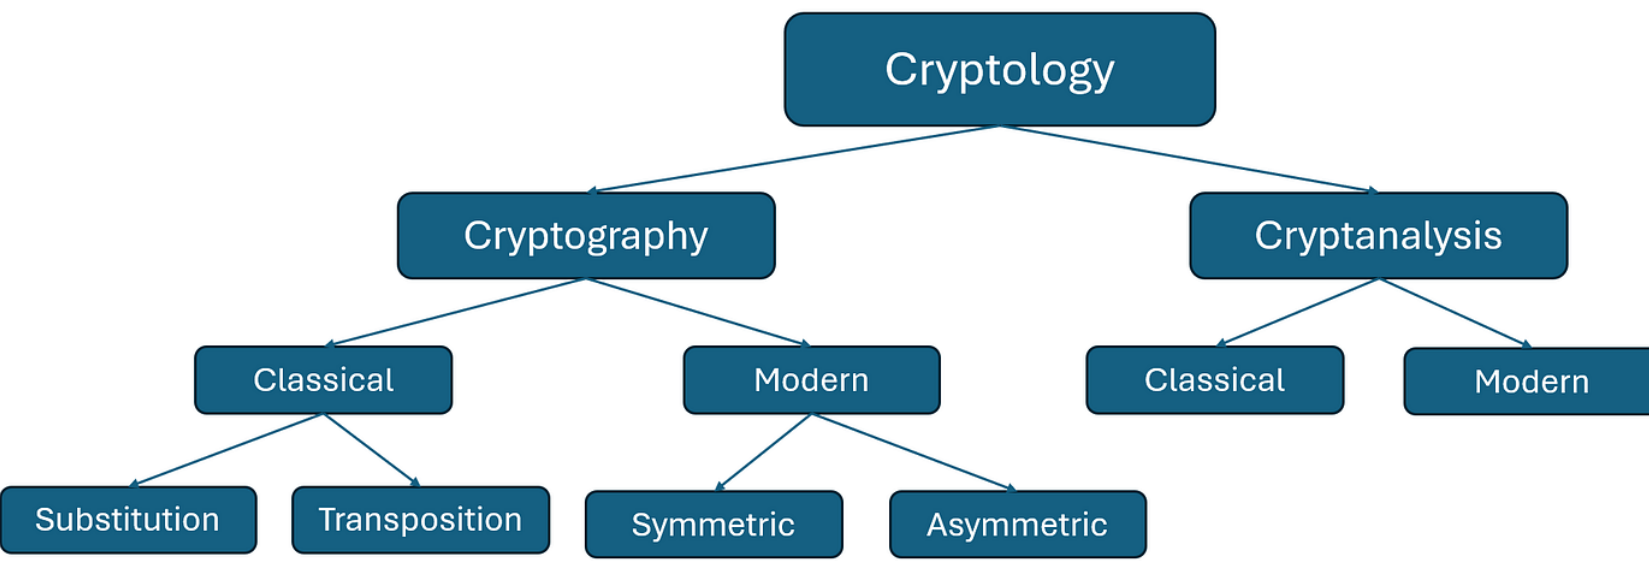
\includegraphics[width=180.39mm,height=154.14mm]{images/llm/page_005_img_01.png}%
\end{textblock*}

\newpage

% --- unit llm 6 ---
% === Halaman 6 (llm) ===

\section*{A. Cipher Substitusi}

\vspace{50.49mm}

\begin{itemize}
    \item Contoh yang terkenal: \textit{Caesar Cipher}
    \item Tiap huruf alfabet digeser 3 huruf ke kanan
\end{itemize}

\vspace{40mm}

\begin{verbatim}
Plainteks  : A B C D E F G H I J K L M N O P Q R S T U V W X Y Z
Cipherteks : D E F G H I J K L M N O P Q R S T U V W X Y Z A B C
\end{verbatim}

\vspace{56.43mm}

\begin{itemize}
    \item Contoh:
    \begin{itemize}
        \item Plainteks: temui saya di jembatan merah nanti malam
        \item Cipherteks: WHPXL VDBD GL MHPEDWDQ PHUDK QDQWL PDODP
    \end{itemize}
\end{itemize}

% deskripsi: Diagram ilustrasi pergeseran huruf alfabet dalam Caesar Cipher, menunjukkan pemetaan huruf A menjadi D, B menjadi E, dan seterusnya.
% bbox normalisasi: [0.5400, 0.2000, 0.9700, 0.3700]
\begin{textblock*}{90.30mm}(113.40mm,59.40mm)
\noindent
\includegraphics[width=90.30mm,height=50.49mm]{images/llm/page_006_img_01.png}%
\end{textblock*}

% deskripsi: Potret patung Julius Caesar, tokoh yang mempopulerkan Caesar Cipher.
% bbox normalisasi: [0.7700, 0.5500, 0.9400, 0.9700]
\begin{textblock*}{35.70mm}(161.70mm,163.35mm)
\noindent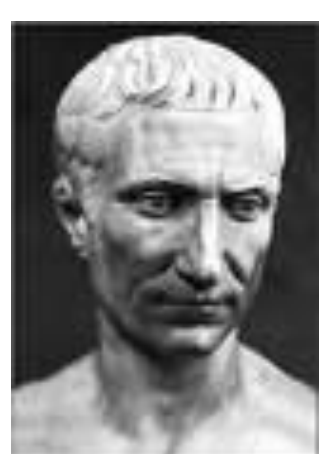
\includegraphics[width=35.70mm,height=124.74mm]{images/llm/page_006_img_02.png}%
\end{textblock*}

% deskripsi: Ilustrasi lukisan bertema Romawi kuno.
% bbox normalisasi: [0.0000, 0.8100, 0.1400, 1.0000]
\begin{textblock*}{29.40mm}(0.00mm,240.57mm)
\noindent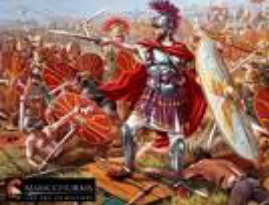
\includegraphics[width=29.40mm,height=56.43mm]{images/llm/page_006_img_03.png}%
\end{textblock*}

\newpage

% --- unit llm 7 ---
% === Halaman 7 (llm) ===

\begin{itemize}
    \item Supaya lebih aman, cipherteks dikelompokkan ke dalam kelompok $n$-huruf, misalnya kelompok 4-huruf:
    
    \noindent Semula: \texttt{WHPXL VDBD GL MHPEDWDQ PHUDK QDQWL PDODP}\\
    Menjadi: \texttt{WHPX LVDB DGLM HPED WDQP HUDK QDQW LPDO DP}
    
    \item Atau membuang semua spasi:
    \[ \texttt{WHPXLVDBDGLMHPEDWDQPHUDKQDQWLPDPDP} \]
    
    \item Tujuannya agar proses kriptanalisis menjadi lebih sulit dilakukan
\end{itemize}

\newpage

% --- unit llm 8 ---
% === Halaman 8 (llm) ===

\begin{itemize}
    \item Enkripsi dan dekripsi Caesar Cipher dapat dilakukan secara matematis
    \item Misalkan setiap huruf alfabet dikodekan ke dalam integer dari 0 sampai 25 sebagai berikut:
\end{itemize}

\vspace{5mm}

\vspace{5mm}

maka, secara matematis Caesar Cipher dirumuskan sebagai:

\[ 
\text{Enkripsi: } c = E(p) = (p + 3) \pmod{26} \\
\text{Dekripsi: } p = D(c) = (c - 3) \pmod{26} 
\]

Ket: $p = \text{plainteks}; \quad c = \text{cipherteks}$

% deskripsi: Tabel pemetaan huruf alfabet (A-Z) ke nilai integer (0-25) untuk Caesar Cipher
% bbox normalisasi: [0.0680, 0.2900, 0.9530, 0.4230]
\begin{textblock*}{185.85mm}(14.28mm,86.13mm)
\noindent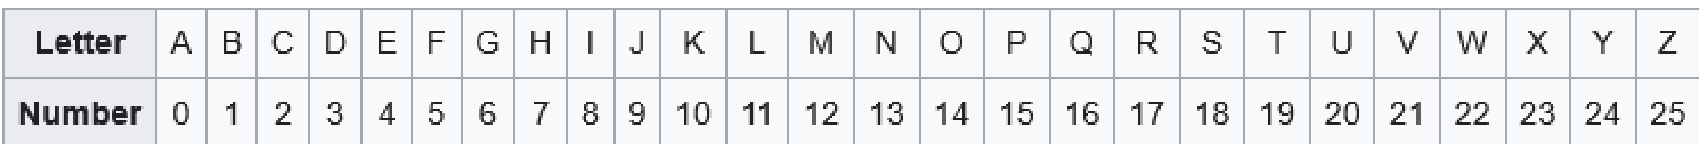
\includegraphics[width=185.85mm,height=39.50mm]{images/llm/page_008_img_01.png}%
\end{textblock*}

\newpage

% --- unit llm 9 ---
% === Halaman 9 (llm) ===

\vspace{21.68mm}

\section*{ENKRIPSI:}

Plainteks: \texttt{temui saya di jembatan merah nanti malam}

\begin{itemize}
    \item $p_1 = \text{'t'} = 19 \rightarrow c_1 = E(19) = (19 + 3) \pmod{26} = 22 = \text{'W'}$
    \item $p_2 = \text{'e'} = 4 \rightarrow c_2 = E(4) = (4 + 3) \pmod{26} = 7 = \text{'H'}$
    \item $p_3 = \text{'m'} = 12 \rightarrow c_3 = E(12) = (12 + 3) \pmod{26} = 15 = \text{'P'}$
    \item $p_4 = \text{'u'} = 20 \rightarrow c_4 = E(20) = (20 + 3) \pmod{26} = 23 = \text{'X'}$
    \item $p_5 = \text{'i'} = 8 \rightarrow c_4 = E(8) = (8 + 3) \pmod{26} = 11 = \text{'L'}$
    \item dst...
\end{itemize}

Cipherteks: \texttt{WHPXL VDBD GL MHPEDWDQ PHUDK QDQWL PDODP}

% deskripsi: Tabel pemetaan huruf alfabet A-Z ke angka 0-25
% bbox normalisasi: [0.4160, 0.0120, 0.9940, 0.0850]
\begin{textblock*}{121.38mm}(87.36mm,3.56mm)
\noindent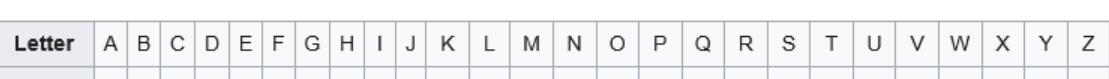
\includegraphics[width=121.38mm,height=21.68mm]{images/llm/page_009_img_01.png}%
\end{textblock*}

\newpage

% --- unit llm 10 ---
% === Halaman 10 (llm) ===

\vspace{31.78mm}

\textbf{DEKRIPSI:}

\vspace{10mm}

Cipherteks: $\text{WHPXL VDBD GL MHPEDWDQ PHUDK QDQWL PDODP}$

\begin{itemize}
    \item $c_1 = \text{'W'} = 22 \rightarrow p_1 = D(22) = (22 - 3) \pmod{26} = 19 = \text{'t'}$
    \item $c_2 = \text{'H'} = 7 \rightarrow p_2 = D(7) = (7 - 3) \pmod{26} = 4 = \text{'e'}$
    \item $c_3 = \text{'P'} = 15 \rightarrow p_3 = D(15) = (15 - 3) \pmod{26} = 12 = \text{'m'}$
    \item $c_4 = \text{'X'} = 23 \rightarrow p_4 = D(23) = (23 - 3) \pmod{26} = 20 = \text{'u'}$
    \item $c_5 = \text{'L'} = 11 \rightarrow p_5 = D(11) = (11 - 3) \pmod{26} = 8 = \text{'i'}$
    \item ...dst
\end{itemize}

\vspace{5mm}

Plainteks: $\text{temui saya di jembatan merah nanti malam}$

% deskripsi: Tabel referensi huruf alfabet dan angka yang bersesuaian (A=0 sampai Z=25).
% bbox normalisasi: [0.3970, 0.0370, 0.9770, 0.1440]
\begin{textblock*}{121.80mm}(83.37mm,10.99mm)
\noindent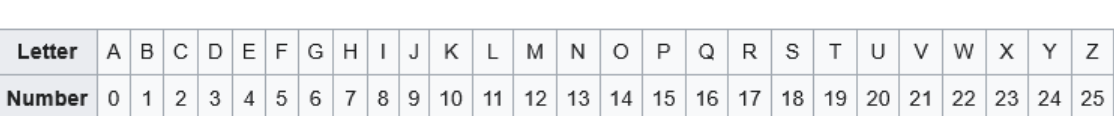
\includegraphics[width=121.80mm,height=31.78mm]{images/llm/page_010_img_01.png}%
\end{textblock*}

\newpage

% --- unit llm 11 ---
% === Halaman 11 (llm) ===

\vspace{150.88mm}

\vspace{80mm}
\begin{center}
\textit{Caesar wheel} untuk membentuk tabel substitusi huruf alfabet
\end{center}

Lihat demo online: \url{https://www.101computing.net/cipher-wheel.html}

% deskripsi: Foto sebuah alat Caesar wheel berwarna emas yang terdiri dari dua lingkaran konsentris dengan huruf alfabet untuk proses enkripsi substitusi.
% bbox normalisasi: [0.2700, 0.2200, 0.6990, 0.7280]
\begin{textblock*}{90.09mm}(56.70mm,65.34mm)
\noindent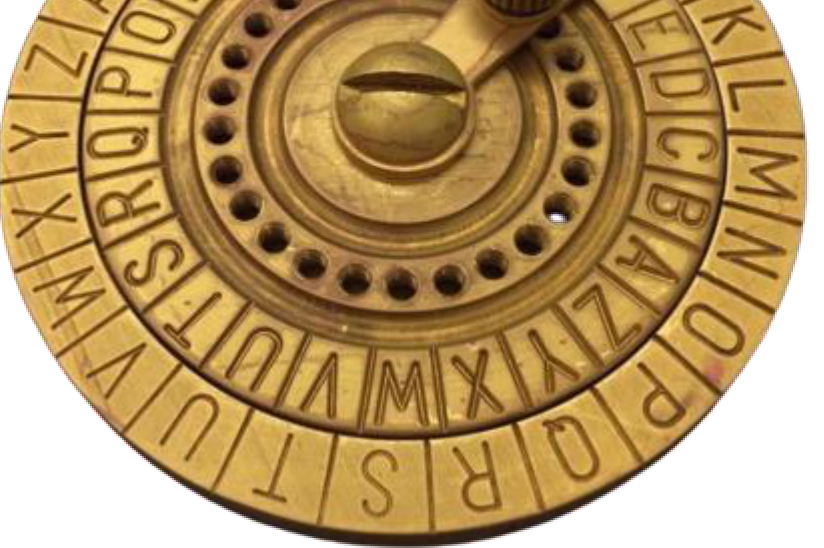
\includegraphics[width=90.09mm,height=150.88mm]{images/llm/page_011_img_01.png}%
\end{textblock*}

\newpage

% --- unit llm 12 ---
% === Halaman 12 (llm) ===

\begin{center}
\textbf{Caesar Cipher Wheel}
\end{center}

\vspace{10mm}

\begin{center}
Enter the key: \textbf{5}
\end{center}

% deskripsi: Ilustrasi interaktif Caesar Cipher Wheel yang menunjukkan dua lingkaran alfabet konsentris untuk enkripsi dan dekripsi teks dengan kunci tertentu.
% bbox normalisasi: [0.3180, 0.2040, 0.6820, 0.8750]
\begin{textblock*}{76.44mm}(66.78mm,60.59mm)
\noindent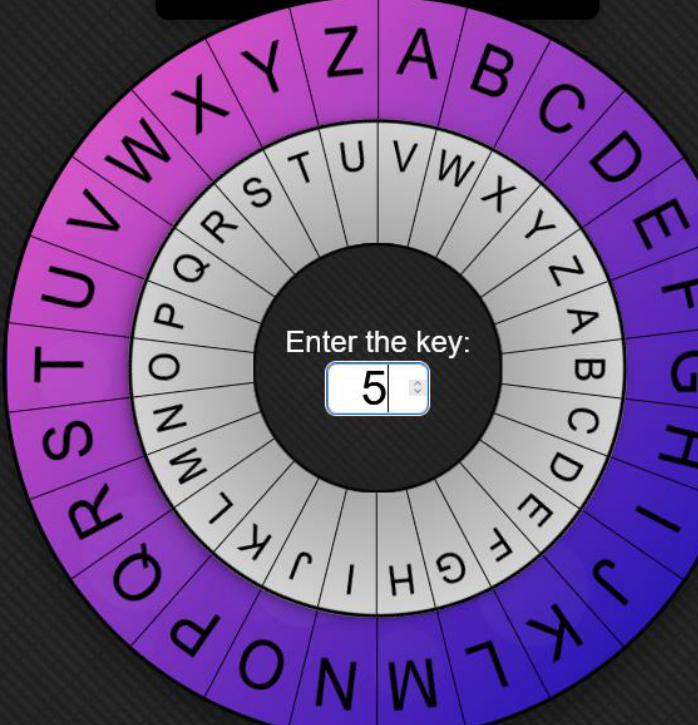
\includegraphics[width=76.44mm,height=199.29mm]{images/llm/page_012_img_01.png}%
\end{textblock*}

\newpage

% --- unit llm 13 ---
% === Halaman 13 (llm) ===

\begin{itemize}
    \item Secara umum, jika pergeseran huruf sejauh $k$, maka:
    
    \begin{align*}
    \text{Enkripsi: } c &= E(p) = (p + k) \pmod{26} \\
    \text{Dekripsi: } p &= D(c) = (c - k) \pmod{26} \\
    k &= \text{kunci rahasia}
    \end{align*}
    
    \item Untuk alfabet berupa 256 karakter ASCII, maka:
    
    \begin{align*}
    \text{Enkripsi: } c &= E(p) = (p + k) \pmod{256} \\
    \text{Dekripsi: } p &= D(c_i) = (c - k) \pmod{256} \\
    k &= \text{kunci rahasia}
    \end{align*}
\end{itemize}

\newpage

% --- unit llm 14 ---
% === Halaman 14 (llm) ===

\section*{Latihan}

Enkripsi kalimat berikut dengan Caesar Cipher, $k = 5$

\begin{center}
ADA RENCANA PENYELUNDUPAN NARKOBA DI BANDARA
\end{center}

Tentukan cipherteksnya

\newpage

% --- unit llm 15 ---
% === Halaman 15 (llm) ===

\vspace{239.98mm}

Demo Caesar Cipher Online: https://cryptii.com/pipes/caesar-cipher\vspace{10mm}

% deskripsi: Screenshot antarmuka situs web Cryptii yang menunjukkan proses enkripsi teks 'The quick brown fox jumps over the lazy dog' menggunakan Caesar cipher dengan shift 8, menghasilkan ciphertext 'Bpm ycqks ycqks jzvw nwf rcuxa wdmz bpm tihg lwo'.
% bbox normalisasi: [0.7700, 0.1340, 0.9020, 0.9420]
\begin{textblock*}{27.72mm}(161.70mm,39.80mm)
\noindent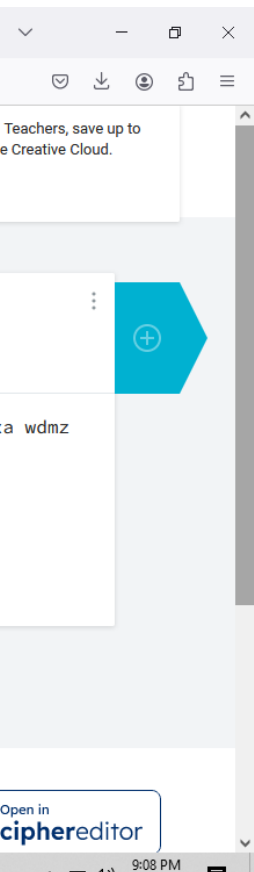
\includegraphics[width=27.72mm,height=239.98mm]{images/llm/page_015_img_01.png}%
\end{textblock*}

\newpage

% --- unit llm 16 ---
% === Halaman 16 (llm) ===

\vspace{106.92mm}

\section*{Program Caesar Cipher dalam Bahasa Python}

\vspace{10mm}

% deskripsi: Screenshot cuplikan kode Python untuk fungsi Caesar\_cipher\_encrypt yang mengimplementasikan enkripsi Caesar Cipher.
% bbox normalisasi: [0.0400, 0.1600, 0.9300, 0.5200]
\begin{textblock*}{186.90mm}(8.40mm,47.52mm)
\noindent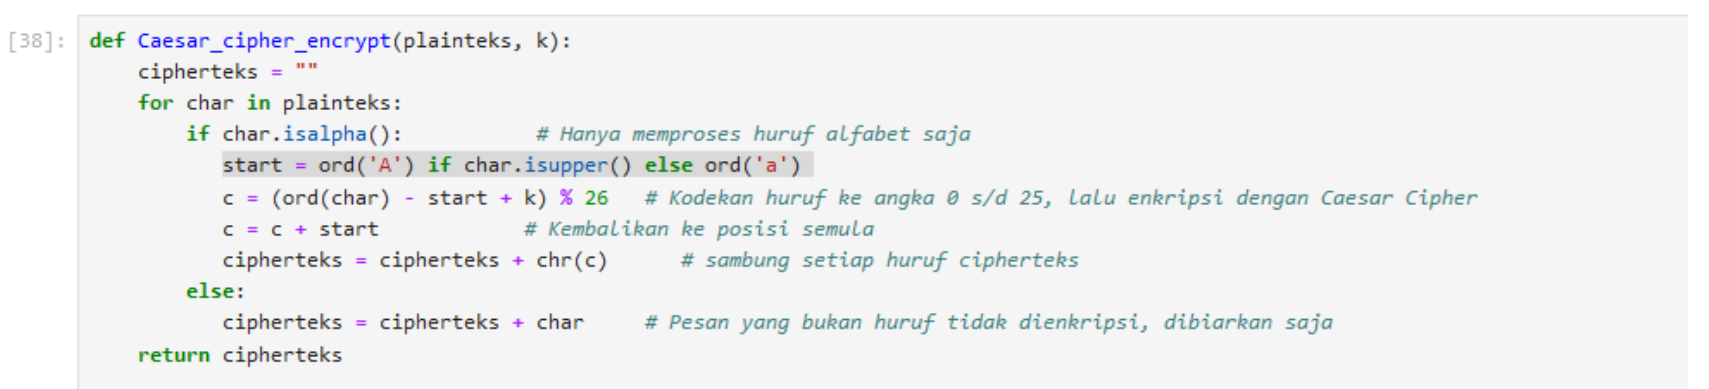
\includegraphics[width=186.90mm,height=106.92mm]{images/llm/page_016_img_01.png}%
\end{textblock*}

% deskripsi: Screenshot cuplikan kode Python untuk fungsi Caesar\_cipher\_decrypt yang mengimplementasikan dekripsi Caesar Cipher.
% bbox normalisasi: [0.0400, 0.5400, 0.9300, 0.9000]
\begin{textblock*}{186.90mm}(8.40mm,160.38mm)
\noindent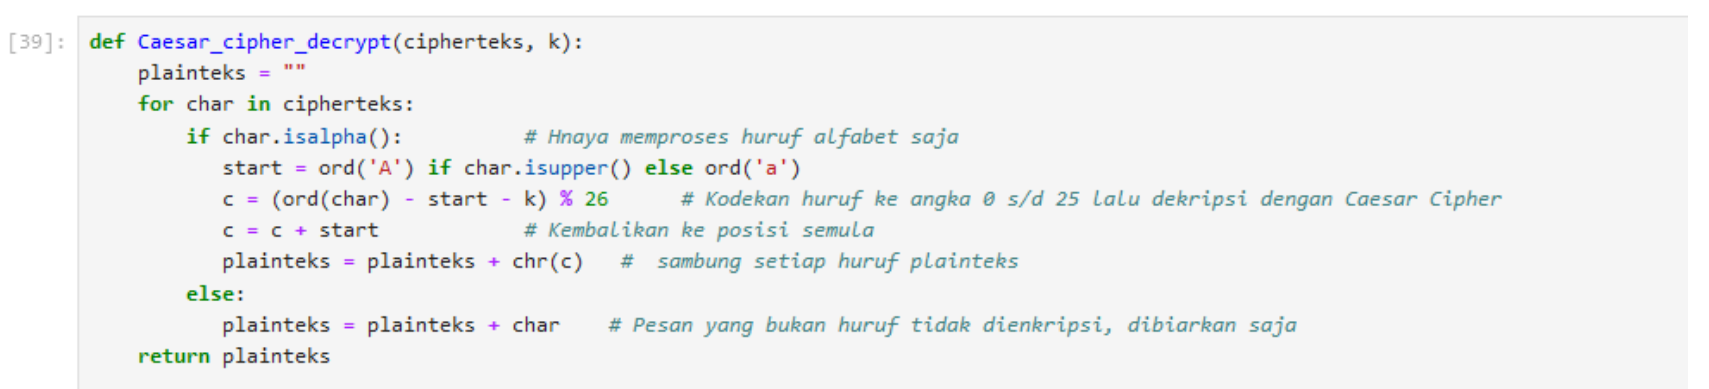
\includegraphics[width=186.90mm,height=106.92mm]{images/llm/page_016_img_02.png}%
\end{textblock*}

\newpage

% --- unit llm 17 ---
% === Halaman 17 (llm) ===

\vspace{214.73mm}

Run program

% deskripsi: Screenshot cuplikan kode Python yang mendemonstrasikan implementasi Caesar Cipher untuk enkripsi dan dekripsi pesan, lengkap dengan input pengguna dan output yang dihasilkan.
% bbox normalisasi: [0.0400, 0.1840, 0.9580, 0.9070]
\begin{textblock*}{192.78mm}(8.40mm,54.65mm)
\noindent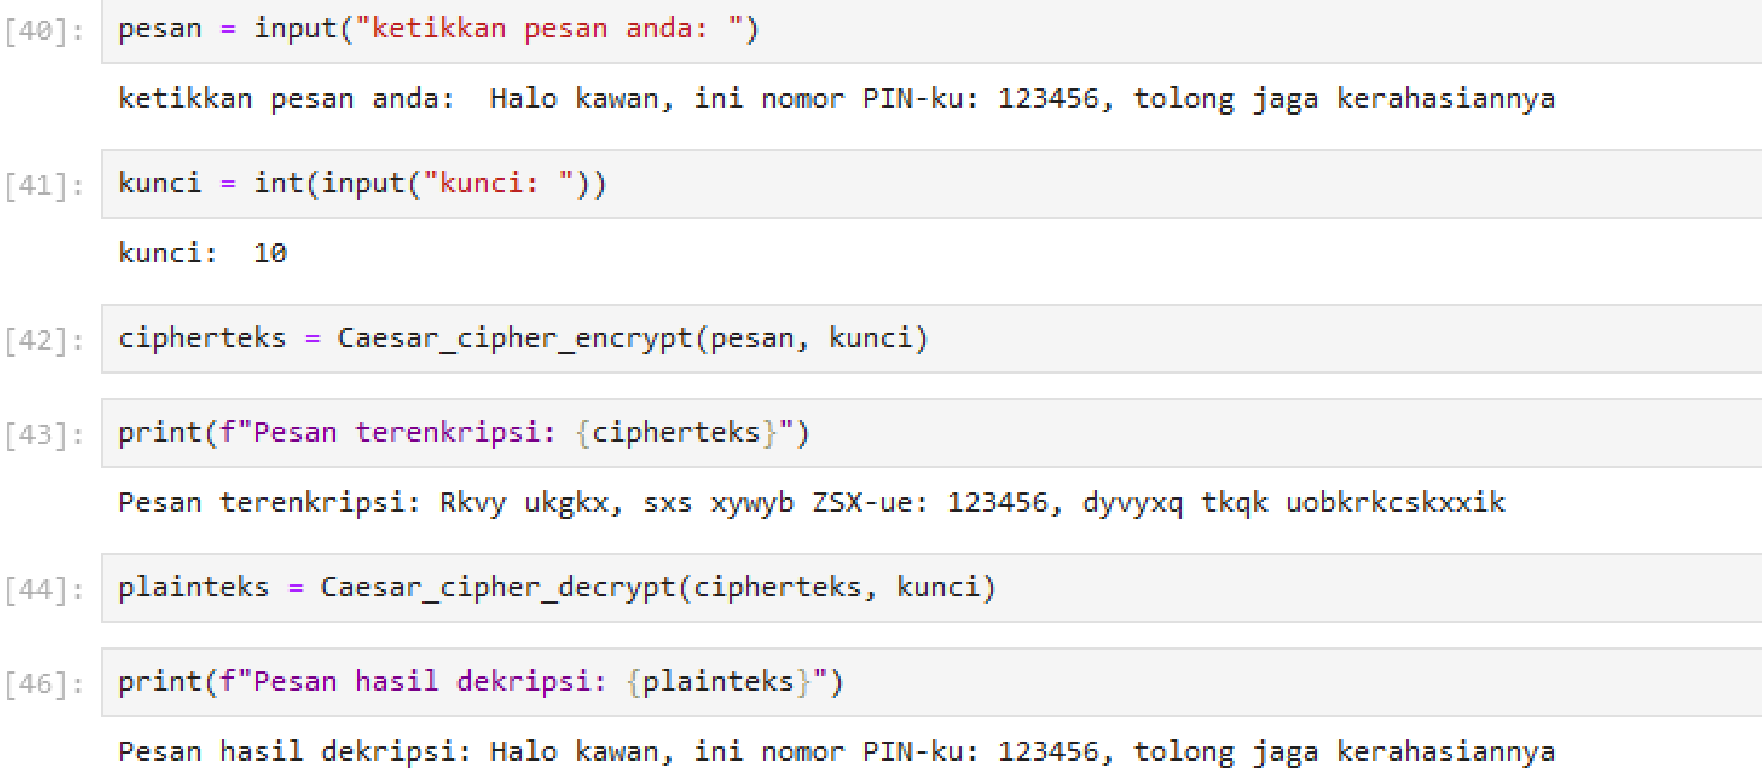
\includegraphics[width=192.78mm,height=214.73mm]{images/llm/page_017_img_01.png}%
\end{textblock*}

\newpage

% --- unit llm 18 ---
% === Halaman 18 (llm) ===

\vspace{154.44mm}

\section*{Program Caesar Cipher dalam Bahasa Python (256 karakter ASCII)}

% deskripsi: Screenshot potongan kode Python untuk fungsi enkripsi dan dekripsi Caesar Cipher menggunakan 256 karakter ASCII.
% bbox normalisasi: [0.0500, 0.2000, 0.9400, 0.7200]
\begin{textblock*}{186.90mm}(10.50mm,59.40mm)
\noindent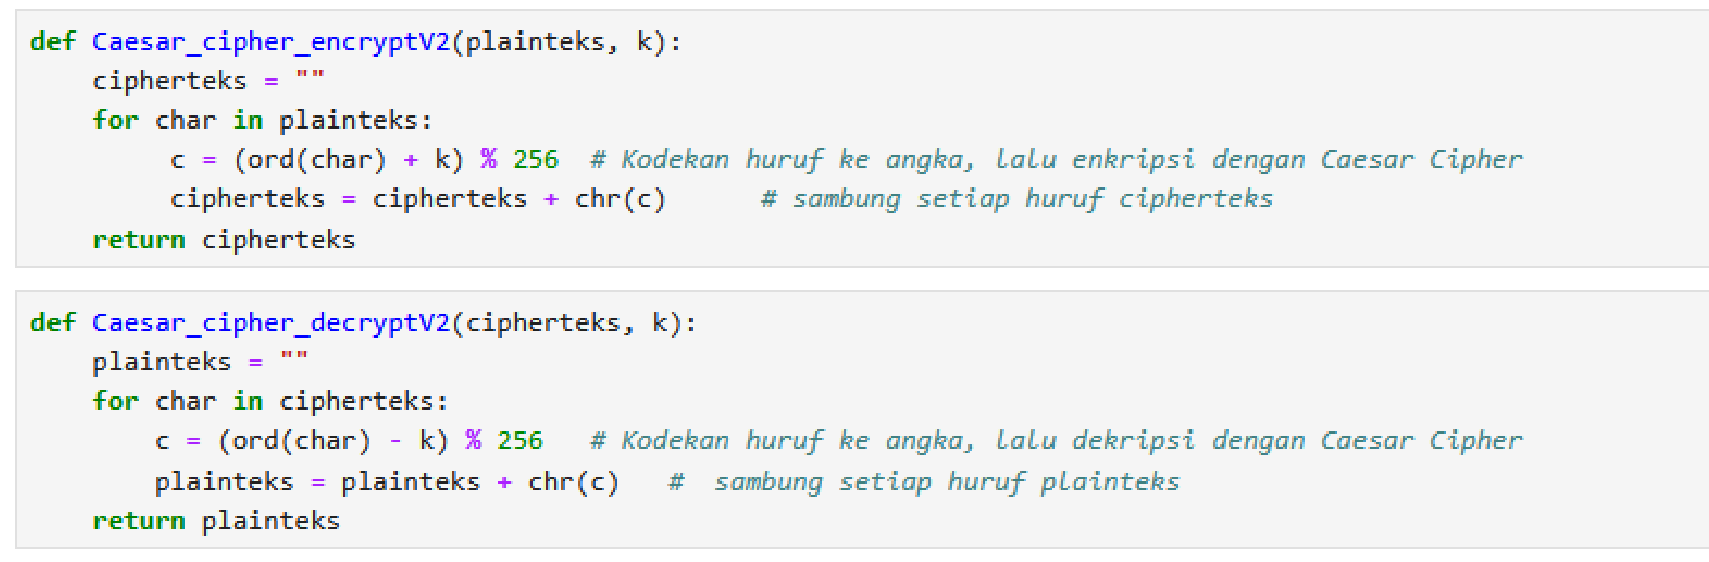
\includegraphics[width=186.90mm,height=154.44mm]{images/llm/page_018_img_01.png}%
\end{textblock*}

\newpage

% --- unit llm 19 ---
% === Halaman 19 (llm) ===

\vspace{209.98mm}

\section*{Run program}

% deskripsi: Screenshot terminal yang menunjukkan eksekusi program Python untuk enkripsi dan dekripsi Caesar Cipher, menampilkan input pesan 'Nomor telponku 08234654890', input kunci '189', hasil ciphertext yang terenkripsi, dan hasil plainteks setelah didekripsi kembali.
% bbox normalisasi: [0.0970, 0.1900, 0.7880, 0.8970]
\begin{textblock*}{145.11mm}(20.37mm,56.43mm)
\noindent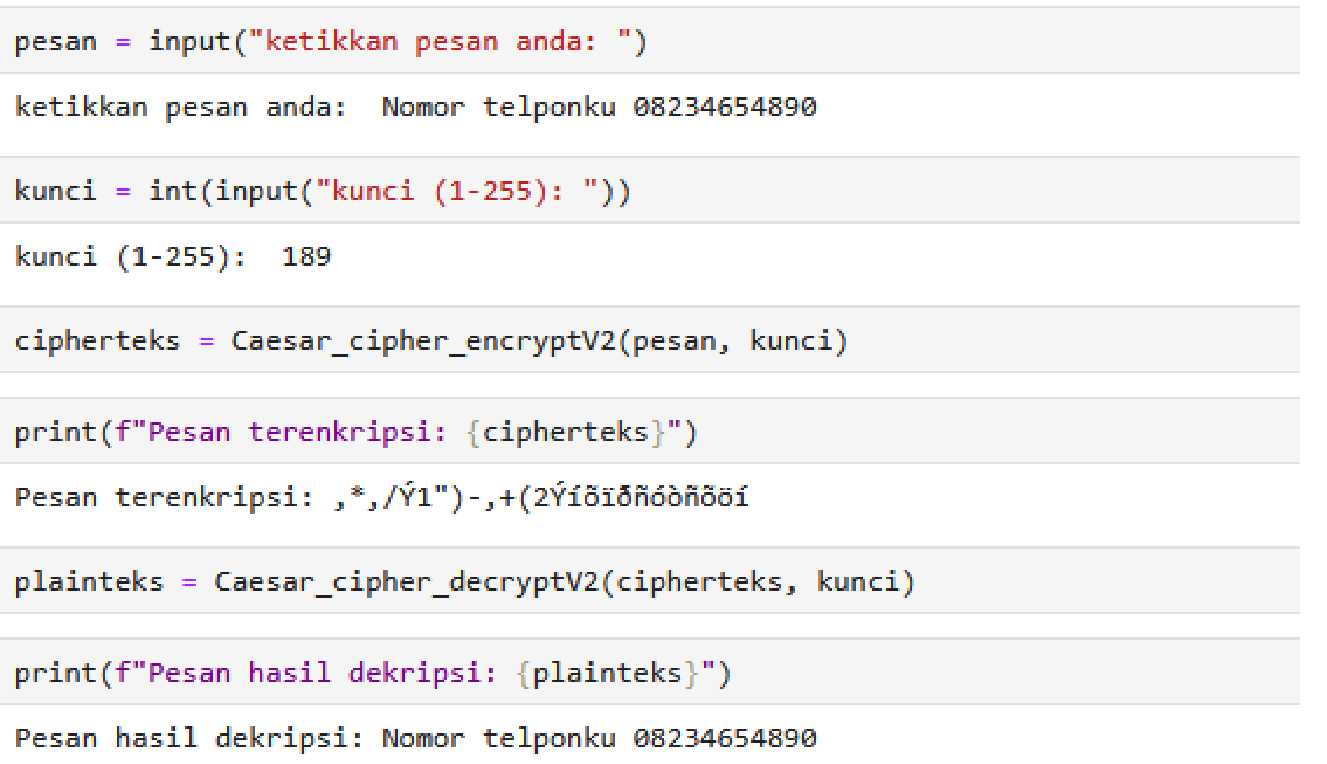
\includegraphics[width=145.11mm,height=209.98mm]{images/llm/page_019_img_01.png}%
\end{textblock*}

\newpage

% --- unit llm 20 ---
% === Halaman 20 (llm) ===

\vspace{261.36mm}

\section*{Program Caesar Cipher dalam Bahasa C++}

% deskripsi: Screenshot potongan kode program C++ untuk enkripsi Caesar Cipher yang mencakup fungsi enkripsi(), input pesan, jumlah pergeseran, dan loop untuk memproses setiap karakter alfabet.
% bbox normalisasi: [0.0400, 0.0900, 0.9200, 0.9700]
\begin{textblock*}{184.80mm}(8.40mm,26.73mm)
\noindent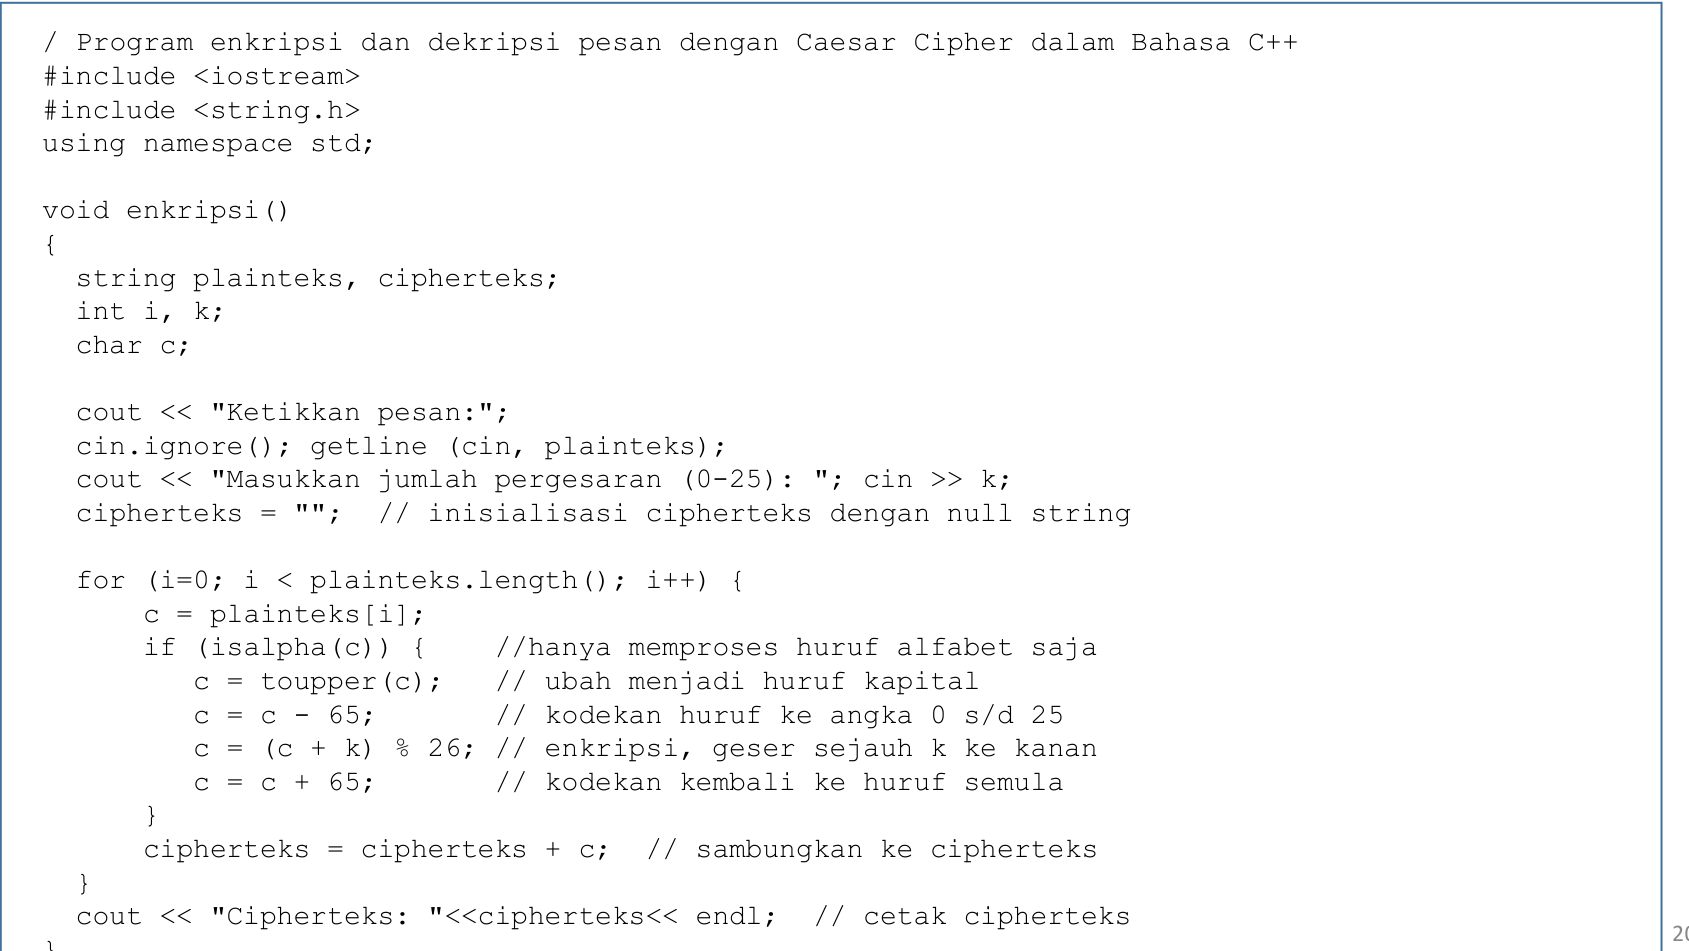
\includegraphics[width=184.80mm,height=261.36mm]{images/llm/page_020_img_01.png}%
\end{textblock*}

\newpage

% --- unit llm 21 ---
% === Halaman 21 (llm) ===

\vspace{273.24mm}

\begin{verbatim}
void dekripsi()
{
    string plainteks, cipherteks;
    int i, k;
    char c;

    cout << "Ketikkan cipherteks: ";
    cin.ignore();getline (cin, cipherteks);
    cout << "Masukkan jumlah pergesaran (0-25): ";
    cin >> k;
    plainteks = ""; // inisialisasi plainteks dengan null string

    for (i=0; i < cipherteks.length(); i++) {
        c = cipherteks[i];
        if (isalpha(c)) {
            //hanya memproses alfabet
            c = toupper(c); // ubah karakter ke huruf besar
            c = c - 65; // kodekan huruf ke angka 0 s/d 25
            if (c - k < 0)
                c = 26 + (c - k); // kasus pembagian bilangan negatif
            else
                c = (c - k) % 26;
            c = c + 65; // kodekan kembali ke huruf semula
            c = tolower(c); // plainteks dinyatakan sebagai huruf kecil
        }
        plainteks = plainteks + c; // sambungkan ke plainteks
    }
    cout << "Plainteks: " << plainteks << endl; // cetak plainteks
}
\end{verbatim}

% deskripsi: Screenshot potongan kode program C++ untuk fungsi dekripsi cipher pergeseran.
% bbox normalisasi: [0.0400, 0.0400, 0.9500, 0.9600]
\begin{textblock*}{191.10mm}(8.40mm,11.88mm)
\noindent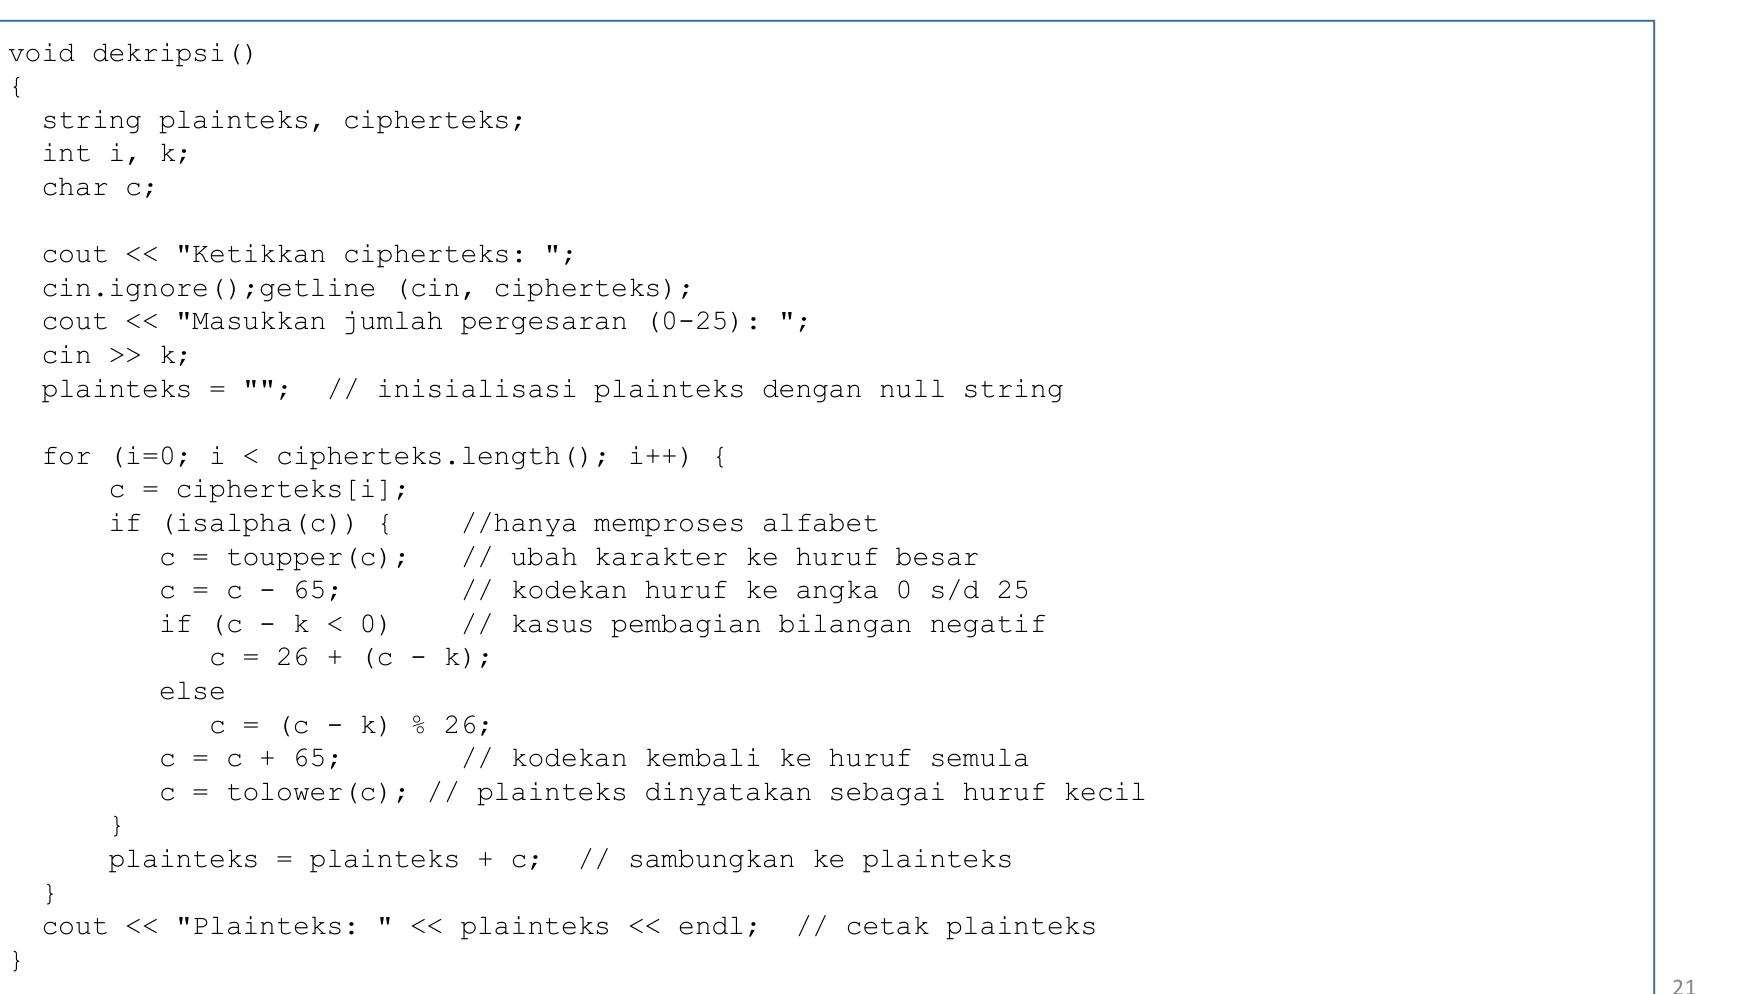
\includegraphics[width=191.10mm,height=273.24mm]{images/llm/page_021_img_01.png}%
\end{textblock*}

\newpage

% --- unit llm 22 ---
% === Halaman 22 (llm) ===

\vspace{193.05mm}

\begin{verbatim}
main()
{
    int pil; bool stop;
    stop = false;

    while (!stop) {
        cout << "Menu: " << endl;
        cout << "1. Enkripsi " << endl;
        cout << "2. Dekripsi " << endl;
        cout << "3. Exit    " << endl;
        cout << "Pilih menu: "; cin >> pil;
        switch (pil) {
            case 1 : enkripsi(); break;
            case 2 : dekripsi(); break;
            case 3 : stop = true; break;
        }
    }
}
\end{verbatim}

% deskripsi: Screenshot potongan kode program C++ yang mengimplementasikan menu pilihan untuk proses enkripsi, dekripsi, dan keluar dari program menggunakan struktur while loop dan switch case.
% bbox normalisasi: [0.0500, 0.0800, 0.4100, 0.7300]
\begin{textblock*}{75.60mm}(10.50mm,23.76mm)
\noindent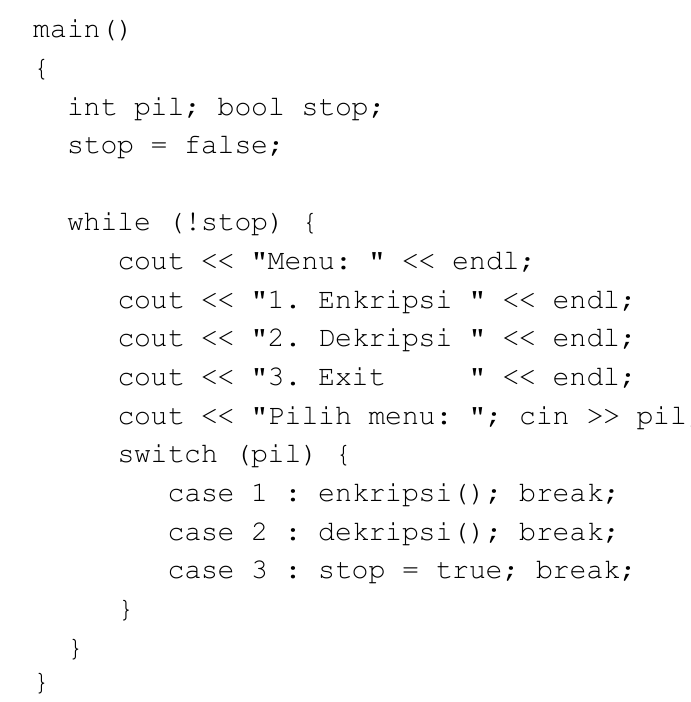
\includegraphics[width=75.60mm,height=193.05mm]{images/llm/page_022_img_01.png}%
\end{textblock*}

\newpage

% --- unit llm 23 ---
% === Halaman 23 (llm) ===

% (tidak ada teks dari model)

% deskripsi: Screenshot Command Prompt Windows yang menunjukkan eksekusi program Caesar Cipher. Terlihat proses enkripsi teks 'the quick brown fox jumps over the lazy dog' dengan pergeseran 18 menjadi 'LZW IMAUC TJGOF XGP BMEHK GNWJ LZW DSRQ UGY', kemudian didekripsi kembali ke teks asli.
% bbox normalisasi: [0.0950, 0.1280, 0.9050, 0.8540]
\begin{textblock*}{170.10mm}(19.95mm,38.02mm)
\noindent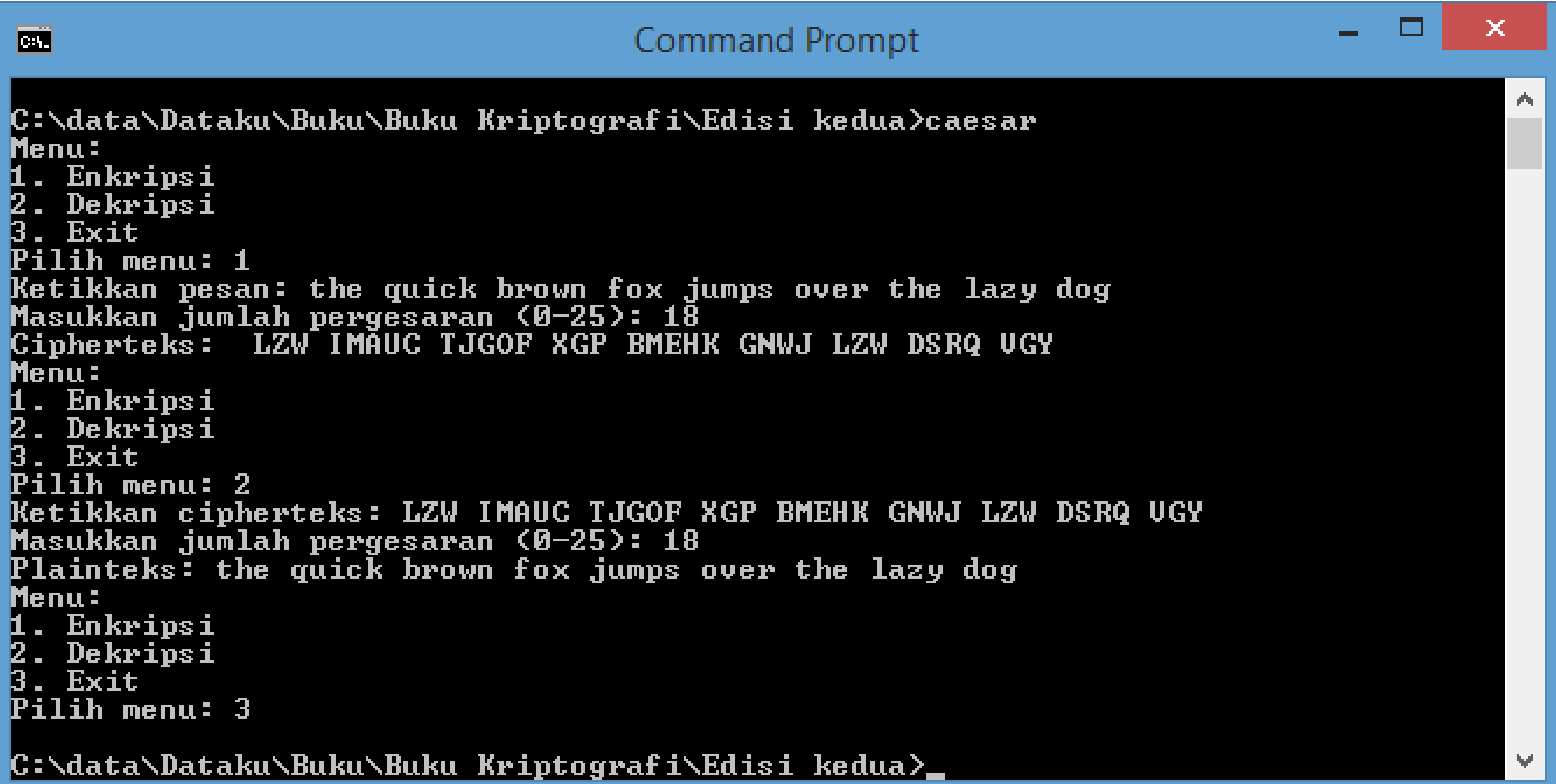
\includegraphics[width=170.10mm,height=215.62mm]{images/llm/page_023_img_01.png}%
\end{textblock*}

\newpage

% --- unit llm 24 ---
% === Halaman 24 (llm) ===

\section*{Kriptanalisis Caesar Cipher}

\begin{itemize}
    \item \textit{Caesar cipher} mudah dipecahkan dengan \textit{exhaustive key search} (\textit{brute force}) karena jumlah kuncinya sangat sedikit (hanya ada 26 kunci).
    \item Coba lakukan dekripsi dengan berbagai nilai $k$ dari 0 sampai 25, lalu periksa apakah hasil dekripsi merupakan kata atau kalimat yang bermakna. Jika ya, maka diduga $k$ adalah kuncinya.
    \item Untuk memastikan $k$ adalah kunci yang benar, maka cobakan $k$ untuk potongan kriptogram lainnya.
\end{itemize}

\newpage

% --- unit llm 25 ---
% === Halaman 25 (llm) ===

Contoh: kriptogram XMZVH

\vspace{5mm}

Plainteks yang potensial adalah CREAM dengan $k = 21$.
Kunci ini digunakan untuk mendekripsikan potongan cipherteks lainnya.

% deskripsi: Tabel contoh exhaustive key search terhadap cipherteks XMZVH yang menunjukkan berbagai kunci (k) ciphering dan hasil dekripsinya.
% bbox normalisasi: [0.1610, 0.2500, 0.8140, 0.6810]
\begin{textblock*}{137.13mm}(33.81mm,74.25mm)
\noindent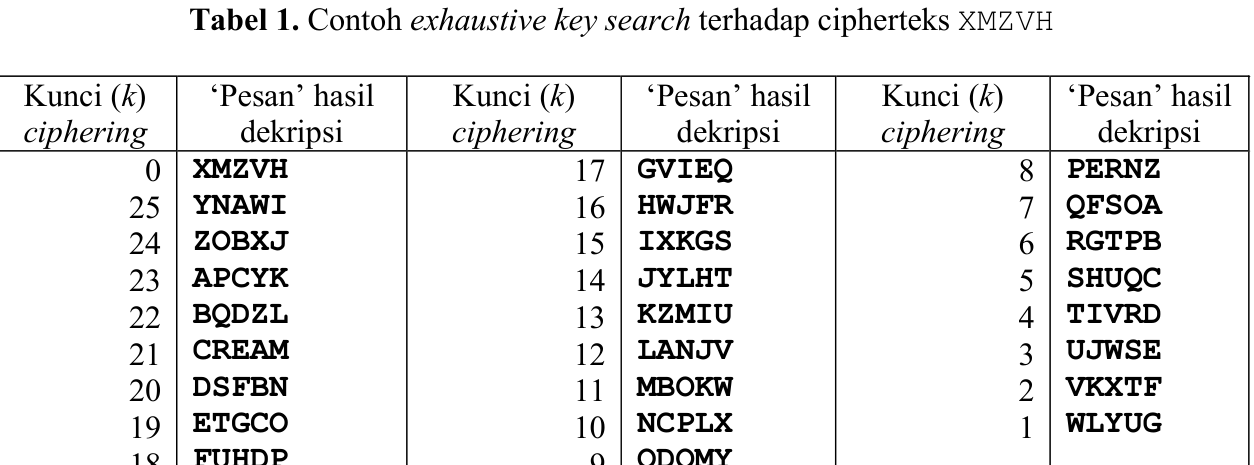
\includegraphics[width=137.13mm,height=128.01mm]{images/llm/page_025_img_01.png}%
\end{textblock*}

\newpage

% --- unit llm 26 ---
% === Halaman 26 (llm) ===

\vspace{193.05mm}

Contoh lain:\
Cipherteks: PHHW PH DIWHU WKH WRJD SDUWB

% deskripsi: Ilustrasi proses dekripsi Caesar Cipher dengan mencoba berbagai nilai kunci (k) untuk menerjemahkan cipherteks menjadi plaintext yang terbaca.
% bbox normalisasi: [0.0900, 0.2000, 0.5600, 0.8500]
\begin{textblock*}{98.70mm}(18.90mm,59.40mm)
\noindent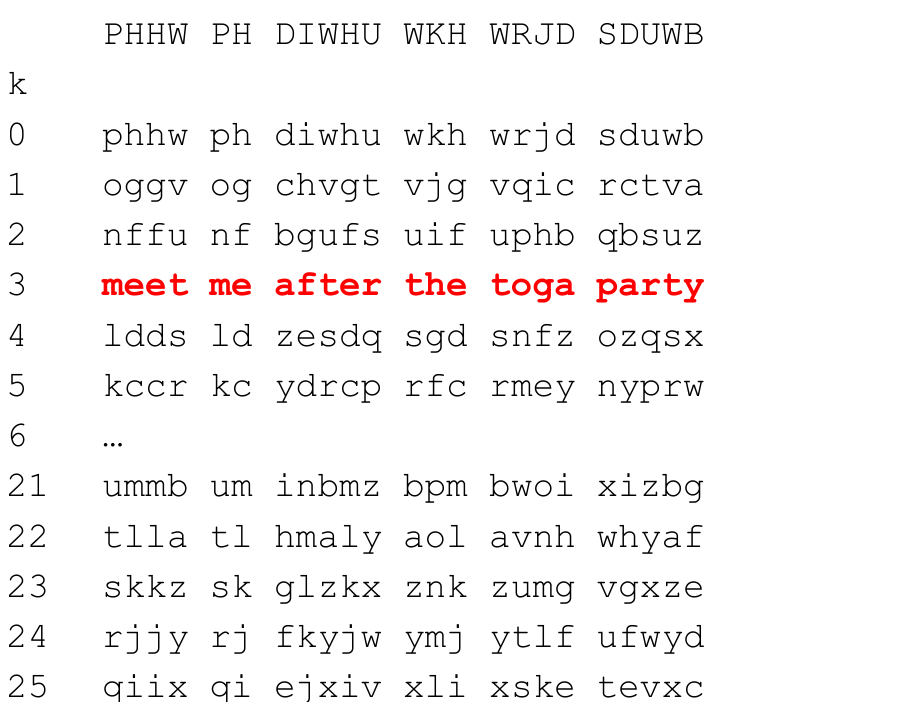
\includegraphics[width=98.70mm,height=193.05mm]{images/llm/page_026_img_01.png}%
\end{textblock*}

\newpage

% --- unit llm 27 ---
% === Halaman 27 (llm) ===

\vspace{241.16mm}

Cipherteks: VIVBQ SQBI SMBMUC LQ ICTI

% deskripsi: Tabel pergeseran kunci k dari 0 sampai 25 dengan hasil dekripsi teks cipher. Baris k=8 ditandai tebal dengan teks 'nanti kita ketemu di aula'.
% bbox normalisasi: [0.2200, 0.1300, 0.6080, 0.9420]
\begin{textblock*}{81.48mm}(46.20mm,38.61mm)
\noindent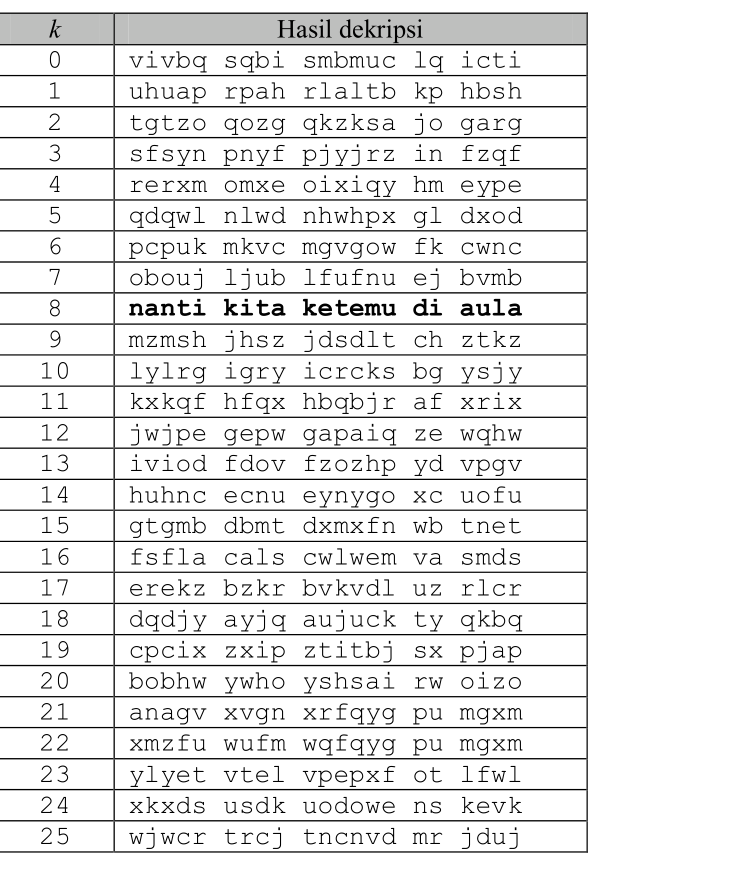
\includegraphics[width=81.48mm,height=241.16mm]{images/llm/page_027_img_01.png}%
\end{textblock*}

\newpage

% --- unit llm 28 ---
% === Halaman 28 (llm) ===

\begin{itemize}
    \item Bagaimana jika terdapat dua atau lebih nilai $k$ yang menghasilkan pesan-pesan bermakna?
\end{itemize}

Contoh: Misalkan kriptogram \texttt{HSPPW} menghasilkan dua kemungkinan kunci yang potensial, yaitu:

\begin{align*}
    k = 4 & \text{ menghasilkan pesan } \texttt{dolls} \quad (\text{boneka}) \\
    k = 11 & \text{ menghasilkan } \texttt{wheel} \quad (\text{roda})
\end{align*}

Nilai $k$ mana yang benar?

Jika kasusnya demikian, maka lakukan dekripsi terhadap potongan cipherteks lain tetapi cukup menggunakan $k = 4$ dan $k = 11$ agar dapat disimpulkan kunci mana yang benar.

\newpage

% --- unit llm 29 ---
% === Halaman 29 (llm) ===

\begin{itemize}
  \item Di dalam sistem operasi Unix, \texttt{ROT13} adalah fungsi menggunakan \textit{Caesar cipher} dengan pergeseran $k = 13$
\end{itemize}

\vspace{60mm}

Sumber gambar: Wikipedia

% deskripsi: Diagram ilustrasi cara kerja ROT13 yang menunjukkan pemetaan huruf alfabet A-M ke N-Z dan contoh enkripsi kata 'HELLO' menjadi 'URYYB'.
% bbox normalisasi: [0.1300, 0.2400, 0.6600, 0.8100]
\begin{textblock*}{111.30mm}(27.30mm,71.28mm)
\noindent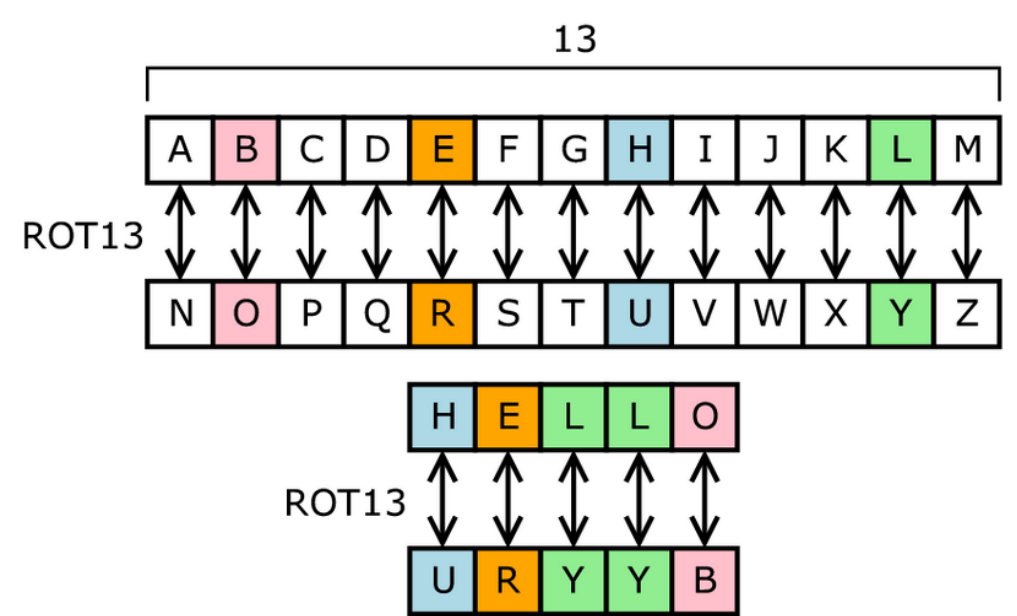
\includegraphics[width=111.30mm,height=169.29mm]{images/llm/page_029_img_01.png}%
\end{textblock*}

\newpage

% --- unit llm 30 ---
% === Halaman 30 (llm) ===

\begin{itemize}
    \item Contoh: $\text{ROT13}(\text{ROTATE}) = \text{EBGNGR}$
    \item Nama ``ROT13'' berasal dari \textit{net.jokes} (\textit{http://groups.google.com/group/net.jokes}) (tahun 1980)
    \item ROT13 biasanya digunakan di dalam forum \textit{online} untuk menyandikan jawaban teka-teki, kuis, canda, dsb
    \item Enkripsi arsip dua kali dengan $\text{ROT13}$ menghasilkan pesan semula:
    \[ P = \text{ROT13}(\text{ROT13}(P)) \]
    sebab $\text{ROT}_{13}(\text{ROT}_{13}(x)) = \text{ROT}_{26}(x) = x$
    \item Jadi dekripsi cukup dilakukan dengan mengenkripsi cipherteks kembali dengan $\text{ROT13}$
\end{itemize}

\newpage

% --- unit llm 31 ---
% === Halaman 31 (llm) ===

\section*{B. Cipher Transposisi}

\begin{itemize}
    \item Cipherteks diperoleh dengan mengubah posisi huruf di dalam plainteks.
    \item Dengan kata lain, algoritma ini melakukan \textit{transpose} terhadap rangkaian huruf di dalam plainteks.
    \item Nama lain untuk metode ini adalah \textit{cipher permutasi}, karena \textit{transpose} setiap karakter di dalam teks sama dengan mempermutasikan karakter-karakter tersebut.
    \item Contoh cipher transposisi: \textit{Columnar Transposition Cipher, Rail Fence Transposition Cipher}
\end{itemize}

\newpage

% --- unit llm 32 ---
% === Halaman 32 (llm) ===

\textbf{1. Columnar Transposition Cipher}

\textbf{Contoh:} Misalkan plainteks adalah

\texttt{sistem dan teknologi informasi itb}

Panjang kunci = 6

\vspace{98.01mm}

\textbf{Enkripsi:}\quad\textcolor{red}{(*buang spasi)}

\vspace{40mm}

\textbf{Cipherteks: (baca secara vertical kolom per kolom)}

SDNIAIAONSSNLFITTOOIEEGRTMKIMB\quad\textcolor{red}{(tanpa spasi)}

SDNI AIAO NSSN LFIT TOOI EEGR TMKI MB\quad\textcolor{red}{(atau blok 4 huruf)}

% deskripsi: Ilustrasi proses enkripsi Columnar Transposition Cipher yang menunjukkan penyusunan teks ke dalam matriks dan arah pembacaan kolom menggunakan tanda panah biru.
% bbox normalisasi: [0.1100, 0.4700, 0.6700, 0.8000]
\begin{textblock*}{117.60mm}(23.10mm,139.59mm)
\noindent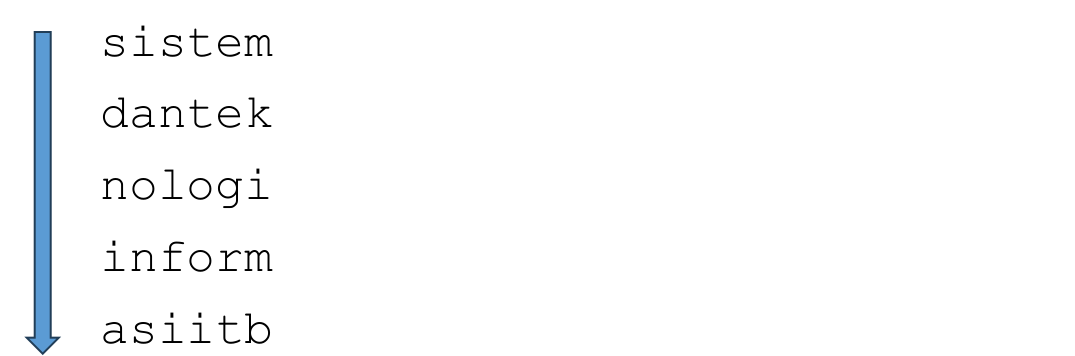
\includegraphics[width=117.60mm,height=98.01mm]{images/llm/page_032_img_01.png}%
\end{textblock*}

\newpage

% --- unit llm 33 ---
% === Halaman 33 (llm) ===

Dekripsi: Bagi panjang cipherteks dengan panjang kunci (Pada contoh ini, $30 / 6 = 5$).\\
Cipherteks: \textcolor{red}{SDNIAIAONSSNLFITTOOIEEGRTMKIMB}\
Tulis cipherteks secara vertical sepanjang 5 kolom:\
\vspace{5mm}
\begin{verbatim}
SDNIA
IAONS
SNLFI
TTOOI
EEGRT
MKIMB
\end{verbatim}
\vspace{5mm}
Plainteks: (baca secara vertikal)\
\texttt{sistemdanteknologiinformasiitb}\
\texttt{sistem dan teknologi informasi itb} \quad (tambahkan spasi)

\newpage

% --- unit llm 34 ---
% === Halaman 34 (llm) ===

\begin{itemize}
    \item Untuk membuat enkripsi menjadi lebih kompleks, gunakan kata kunci sepanjang $n$ dengan huruf-huruf berbeda. Urutan huruf di dalam kata kunci menentukan urutan pembacaan secara vertikal.
    \item Contoh: kata kunci = TOMBAK (urutan huruf sesuai alfabet: 6 5 4 2 1 3)
\end{itemize}

Plainteks: sistem dan teknologi informasi itb

\vspace{124.74mm}

Enkripsi:

\vspace{10mm}

Cipherteks: (baca secara vertikal sesuai urutan huruf di dalam kata kunci $\to 5, 4, 6, 3, 2, 1$)
\textcolor{red}{EEGRTTTOOIMKIMBSNLFIIAONSSDNIA}

% deskripsi: Ilustrasi proses enkripsi kolom dengan kata kunci TOMBAK, menunjukkan pemetaan huruf plainteks ke dalam grid berdasarkan kata kunci.
% bbox normalisasi: [0.1400, 0.4400, 0.2500, 0.8600]
\begin{textblock*}{23.10mm}(29.40mm,130.68mm)
\noindent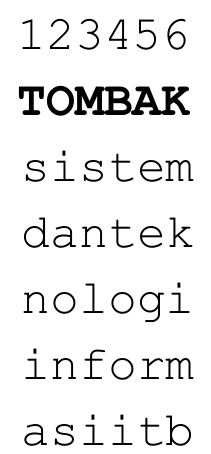
\includegraphics[width=23.10mm,height=124.74mm]{images/llm/page_034_img_01.png}%
\end{textblock*}

\newpage

% --- unit llm 35 ---
% === Halaman 35 (llm) ===

\vspace{237.60mm}

Demo online: \href{https://www.dcode.fr/columnar-transposition-cipher}{https://www.dcode.fr/columnar-transposition-cipher}

% deskripsi: Screenshot halaman web dCode yang menampilkan alat Decoder dan Encoder untuk Columnar Transposition Cipher, lengkap dengan input teks, kunci permutasi, dan opsi konfigurasi.
% bbox normalisasi: [0.0500, 0.1500, 0.8700, 0.9500]
\begin{textblock*}{172.20mm}(10.50mm,44.55mm)
\noindent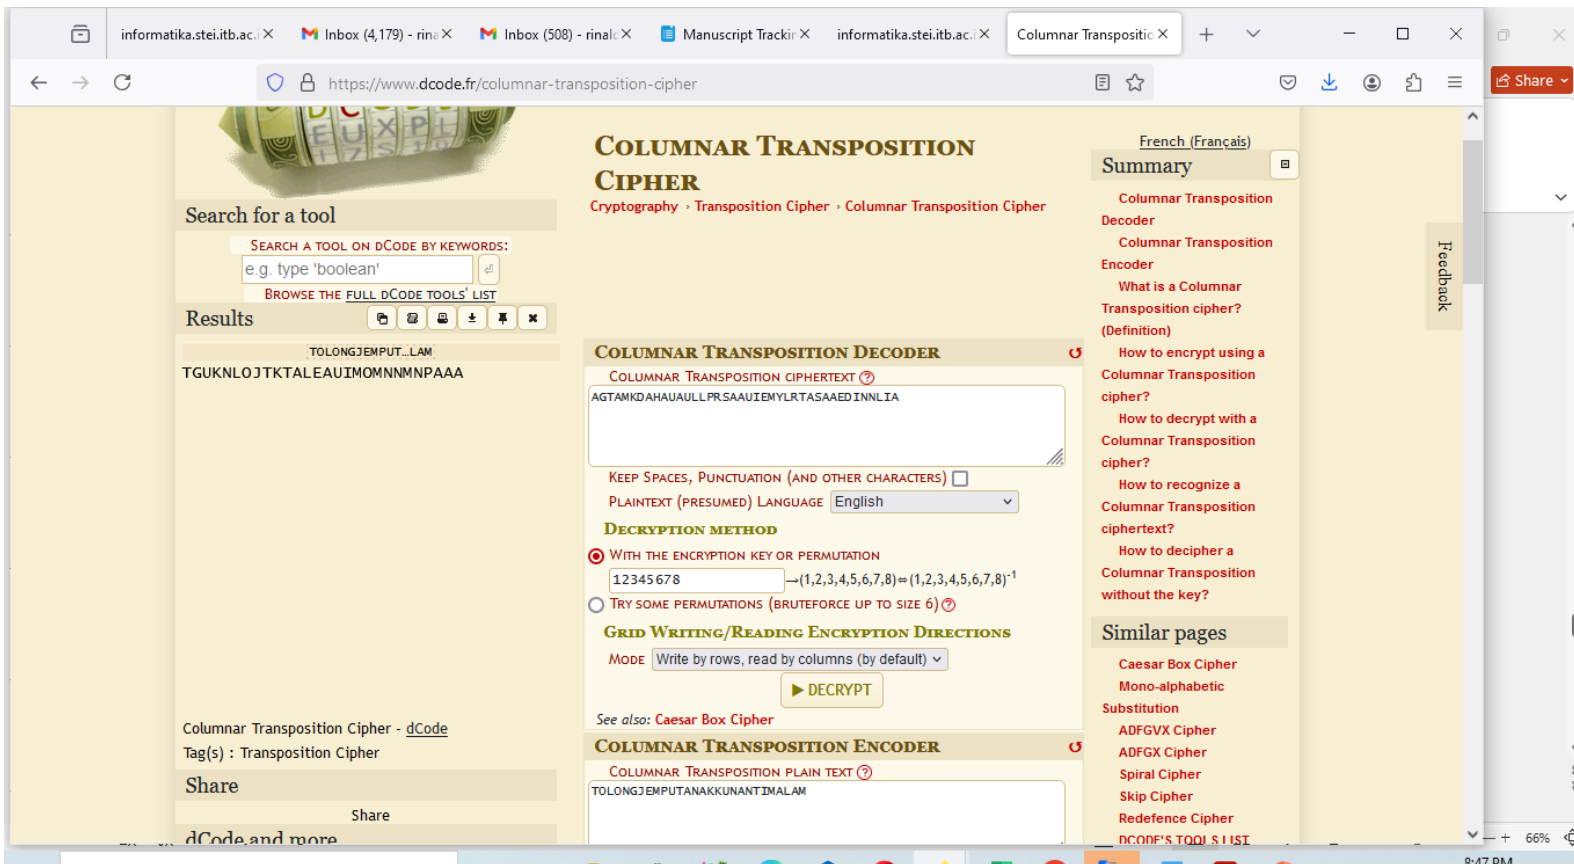
\includegraphics[width=172.20mm,height=237.60mm]{images/llm/page_035_img_01.png}%
\end{textblock*}

\newpage

% --- unit llm 36 ---
% === Halaman 36 (llm) ===

\section*{Program Transposition Cipher dalam Bahasa Python (26 huruf alfabet)}

\begin{verbatim}
import math

def transposition_cipher_encrypt(plaintext, k):
    ciphertext = [''] * k    # membuat sebuah list dengan panjang k, yang setiap
                               # elemennya berupa string kosong.

    for kolom in range(k):
        index = kolom
        while index < len(plaintext):
            ciphertext[kolom] = ciphertext[kolom] + plaintext[index]
            index = index + k
    return ''.join(ciphertext)
\end{verbatim}

\newpage

% --- unit llm 37 ---
% === Halaman 37 (llm) ===

\begin{verbatim}
def transposition_cipher_decrypt(ciphertext, k):
    jumlah_baris = math.ceil(len(ciphertext) / k)
    jumlah_sel_kosong = (jumlah_baris * k) - len(ciphertext)

\vspace{209.38mm}

    plaintext = [''] * jumlah_baris    # membuat sebuah list dengan panjang k, yang
                                       # setiap elemennya berupa string kosong.

    kolom = 0
    baris = 0

    for karakter in ciphertext:
        plaintext[baris] = plaintext[baris] + karakter
        baris = baris + 1

        if (baris == jumlah_baris) or (baris == jumlah_baris-1 and
            kolom >= k - jumlah_sel_kosong):

            baris = 0
            kolom += 1

    return ''.join(plaintext)
\end{verbatim}

% deskripsi: Screenshot potongan kode Python untuk fungsi dekripsi transposition cipher.
% bbox normalisasi: [0.0480, 0.1100, 0.8970, 0.8150]
\begin{textblock*}{178.29mm}(10.08mm,32.67mm)
\noindent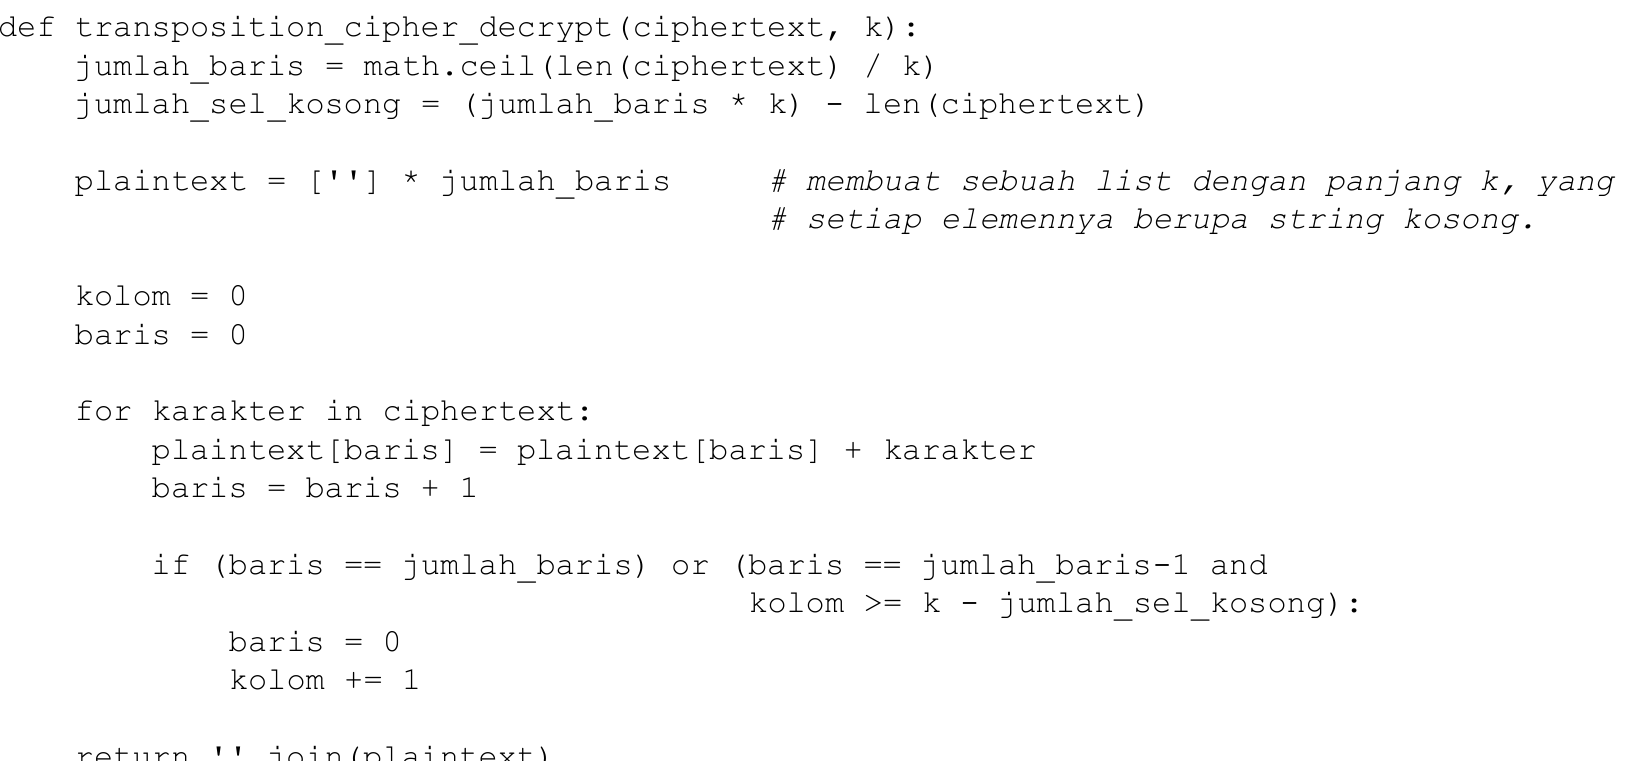
\includegraphics[width=178.29mm,height=209.38mm]{images/llm/page_037_img_01.png}%
\end{textblock*}

\newpage

% --- unit llm 38 ---
% === Halaman 38 (llm) ===

\vspace{225.72mm}

Run program

% deskripsi: Screenshot kode program Python untuk enkripsi dan dekripsi menggunakan transposition cipher beserta output eksekusinya.
% bbox normalisasi: [0.0900, 0.1300, 0.8600, 0.8900]
\begin{textblock*}{161.70mm}(18.90mm,38.61mm)
\noindent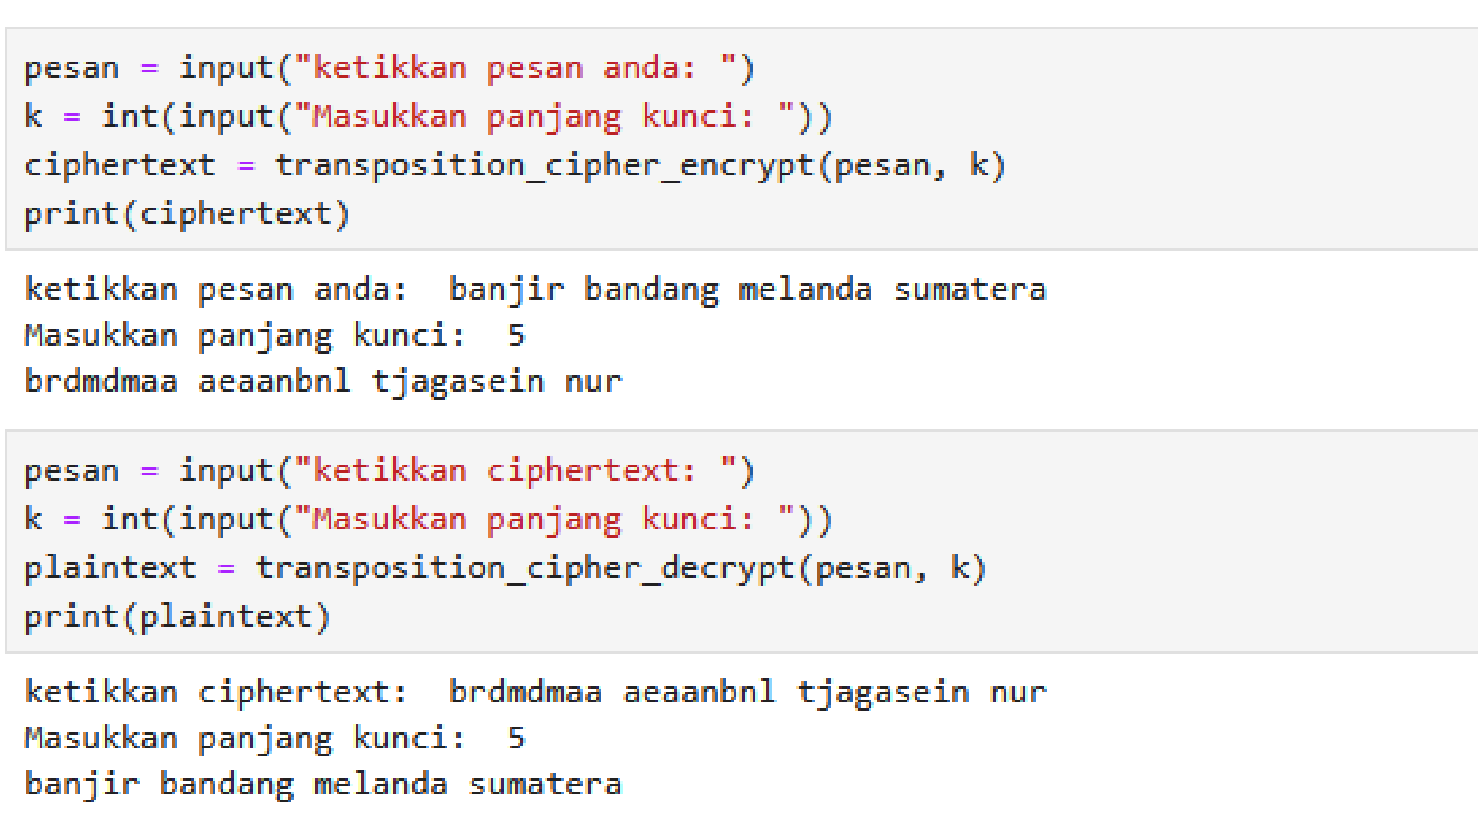
\includegraphics[width=161.70mm,height=225.72mm]{images/llm/page_038_img_01.png}%
\end{textblock*}

\newpage

% --- unit llm 39 ---
% === Halaman 39 (llm) ===

\section*{2. Rail Fence Transposition Cipher}

\textbf{Contoh lain.} Misalkan plainteks adalah

\begin{center}
CRYPTOGRAPHY AND DATA SECURITY
\end{center}

Plainteks disusun menjadi 3 baris ($k = 3$) seperti di bawah ini:

\vspace{10mm}

maka cipherteksnya adalah

\begin{center}
CTAAAEIRPORPYNDTSCRTYGHDAUY
\end{center}

% deskripsi: Ilustrasi penyusunan huruf plainteks dalam pola zigzag 3 baris untuk Rail Fence Cipher
% bbox normalisasi: [0.1700, 0.5200, 0.7400, 0.6600]
\begin{textblock*}{119.70mm}(35.70mm,154.44mm)
\noindent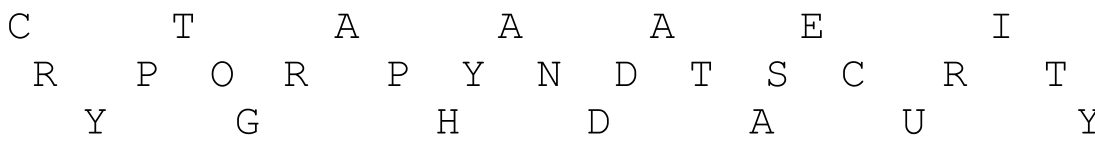
\includegraphics[width=119.70mm,height=41.58mm]{images/llm/page_039_img_01.png}%
\end{textblock*}

\newpage

% --- unit llm 40 ---
% === Halaman 40 (llm) ===

\begin{itemize}
    \item Kita pun dapat membuat variasi cipher transposisi dengan atutan yang kita definisikan sendiri.
    \item Contohnya seperti berikut. Misalkan plainteks: \texttt{ITB GANESHA SEPULUH}
    \item Bagi menjadi blok-blok 8-huruf. Jika $< 8$, tambahkan huruf \textit{dummy}.
\end{itemize}

\vspace{50mm}

\begin{itemize}
    \item Cipherteks: \textbf{STBAGNEIUASPEULHGABDCEFH}
\end{itemize}

% deskripsi: Diagram proses enkripsi transposition cipher yang menunjukkan pemetaan huruf-huruf dari blok plainteks ke urutan baru untuk membentuk cipherteks.
% bbox normalisasi: [0.1050, 0.4450, 0.9050, 0.7450]
\begin{textblock*}{168.00mm}(22.05mm,132.16mm)
\noindent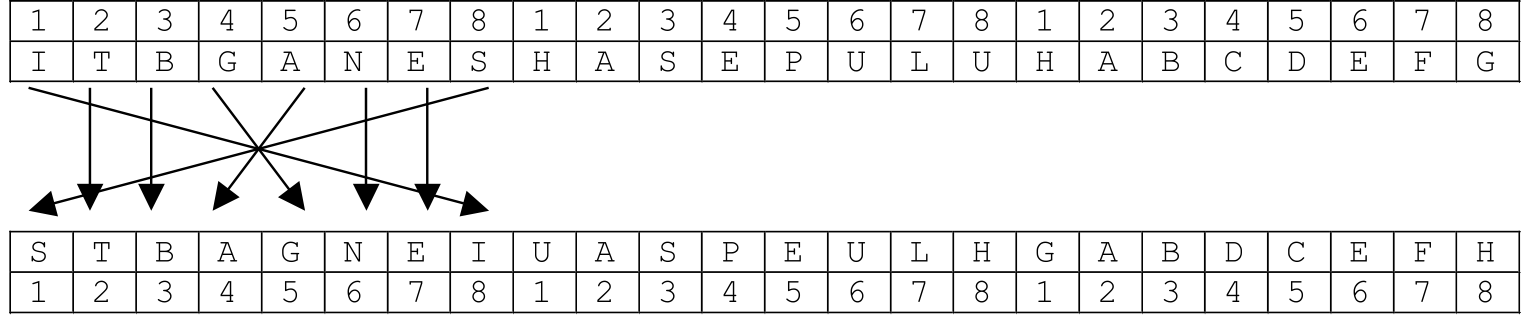
\includegraphics[width=168.00mm,height=89.10mm]{images/llm/page_040_img_01.png}%
\end{textblock*}

\newpage

% --- unit llm 41 ---
% === Halaman 41 (llm) ===

\section*{Super-enkripsi}

\begin{itemize}
    \item Menggabungkan \textit{cipher} substitusi dengan \textit{cipher} transposisi.
    \item Disebut juga \textit{product cipher}
    \item Mula-mula pesan dienkripsi dengan \textit{cipher} substitusi, selanjutnya hasilnya dienkripsi dengan \textit{cipher} transposisi (atau sebaliknya).
\end{itemize}

\textbf{Contoh.} Plainteks \texttt{hello world}

\begin{itemize}
    \item[$\checkmark$] Mula-mula dienkripsi dengan \textit{caesar cipher} ($k = 3$) menjadi \texttt{KHOOR ZRUOG}
    \item[$\checkmark$] kemudian hasil ini dienkripsi lagi dengan \textit{cipher} transposisi ($k = 4$):
\end{itemize}

\vspace{10mm}

\begin{itemize}
    \item \textit{Cipher} modern menggunakan konsep kombinasi \textit{cipher} substitusi dan \textit{cipher} transposisi, namun operasinya dibuat sekompleks mungkin
\end{itemize}

% deskripsi: Ilustrasi proses enkripsi transposisi dari teks KHOOR ZRUOG menjadi cipherteks akhir KROHZGZOUZ
% bbox normalisasi: [0.1300, 0.6400, 0.7400, 0.7900]
\begin{textblock*}{128.10mm}(27.30mm,190.08mm)
\noindent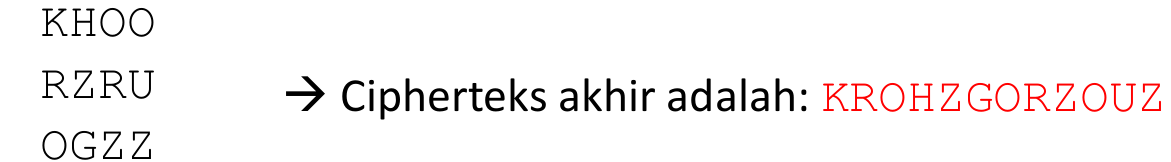
\includegraphics[width=128.10mm,height=44.55mm]{images/llm/page_041_img_01.png}%
\end{textblock*}

\newpage

% --- unit llm 42 ---
% === Halaman 42 (llm) ===

Bersambung

\end{document}
